\subsection{Gráfico}
\label{sec:grafico-funcao-polinomial}

Quando se deseja traçar o gráfico, ao menos um esboço, de uma função polinomial qualquer 
$p(x) = a_n x^n+ a_{n-1} x^{n-1} + \dots + a_1x + a_0$, certas informações são de grande utilidade. 
Algumas delas são:
%
\begin{itemize}
  \item Se $n$ é par, então para $\modu x $ suficientemente grande,
  $p(x)$ tem o mesmo sinal de $a_n$;
  \item Se $n$ é ímpar, então $p(x)$ tem o mesmo sinal de $a_n$ para
  valores positivos  muito grandes de $x$ e tem o sinal oposto de
  $a_n$ para valores negativos muito grandes, em módulo, de $x$.
\end{itemize}

\begin{example}
Sejam $p_1$, $p_2$, $p_3$ e $p_4$ funções polinomiais, cujos gráficos são mostrados nas Imagens
\ref{fig:polinomio-identidade}, \ref{fig:polinomio-quadratico}, \ref{fig:polinomio-cubico} e \ref{fig:polinomio-quartico}.

\begin{figure}[H]
  \centering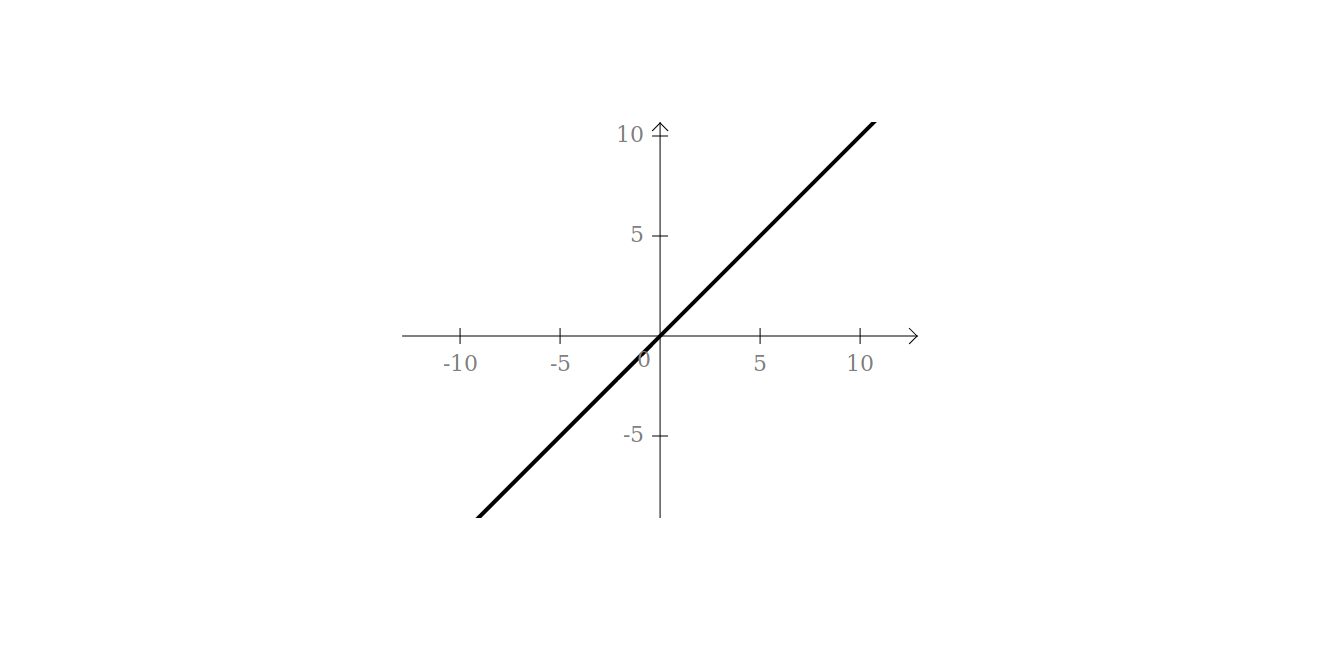
\includegraphics[scale=0.30]{\imgdirfromsection/polinomio-identidade.png}
  \caption{Gráfico da função $p_1$.}
  \label{fig:polinomio-identidade}
\end{figure}

\begin{figure}[H]
  \centering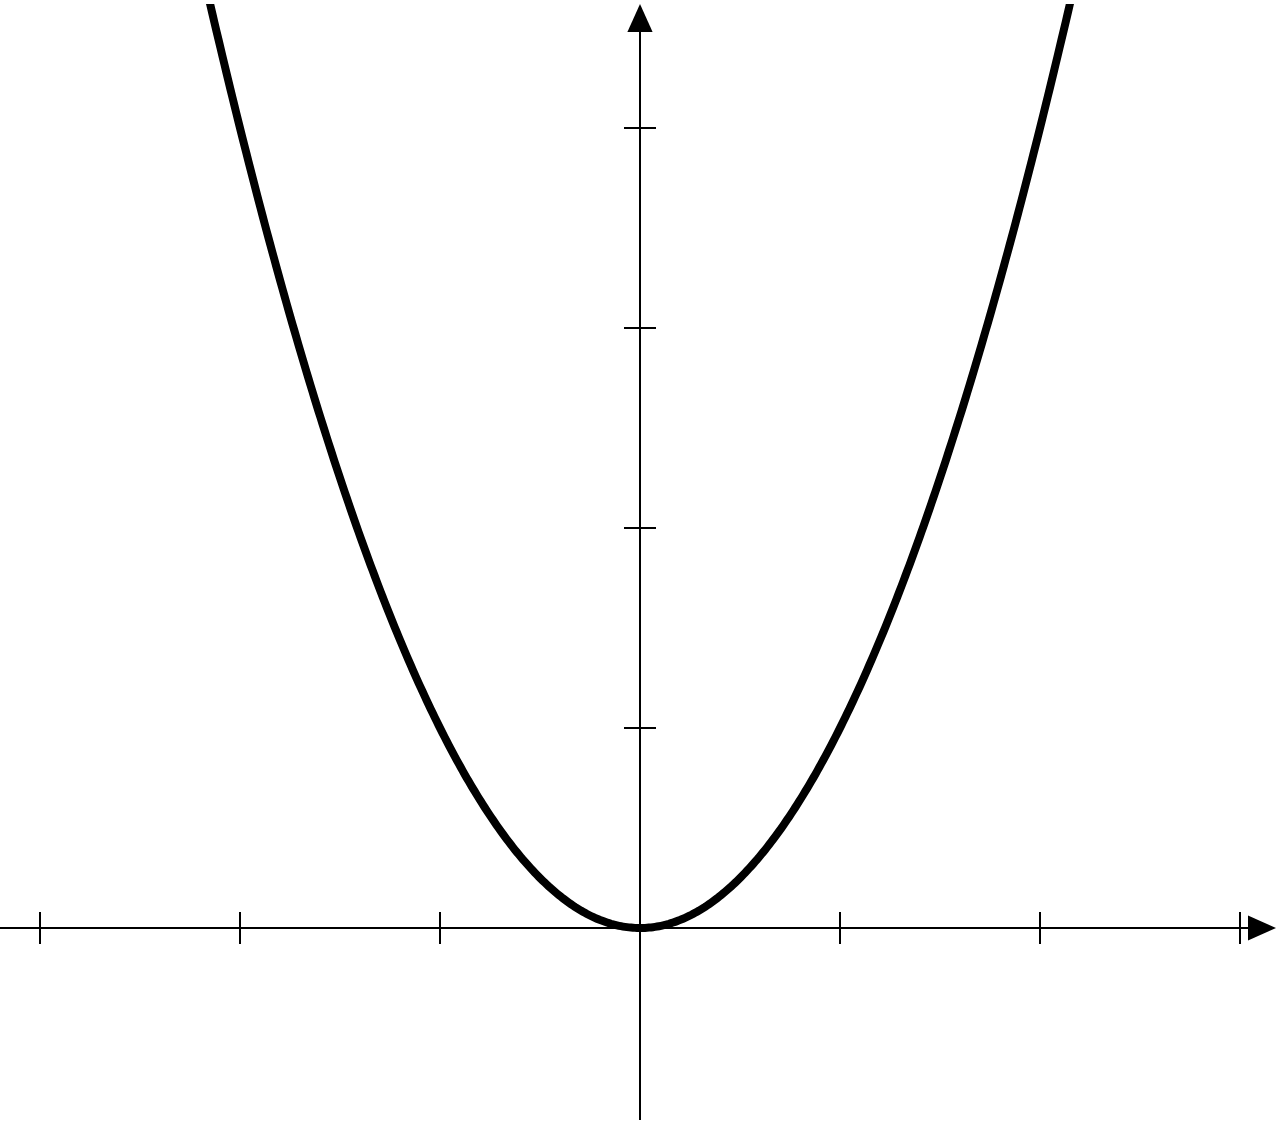
\includegraphics[scale=0.30]{\imgdirfromsection/polinomio-quadratico.png}
  \caption{Gráfico da função $p_2$.}
  \label{fig:polinomio-quadratico}
\end{figure}

\begin{figure}[H]
  \centering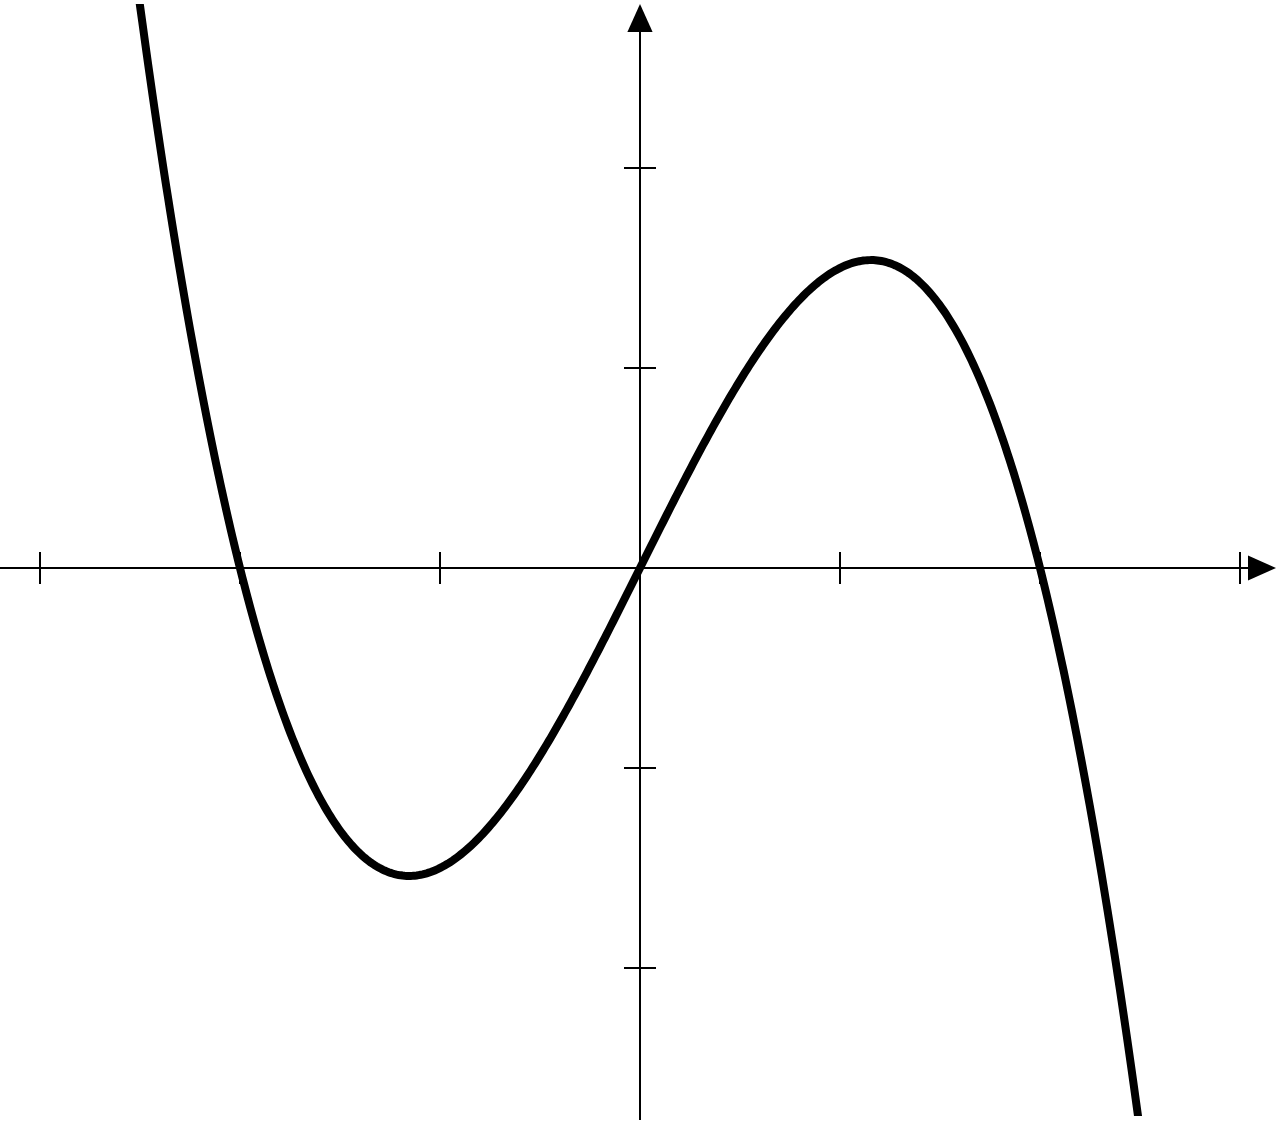
\includegraphics[scale=0.30]{\imgdirfromsection/polinomio-cubico.png}
  \caption{Gráfico da função $p_3$.}
  \label{fig:polinomio-cubico}
\end{figure}

\begin{figure}[H]
  \centering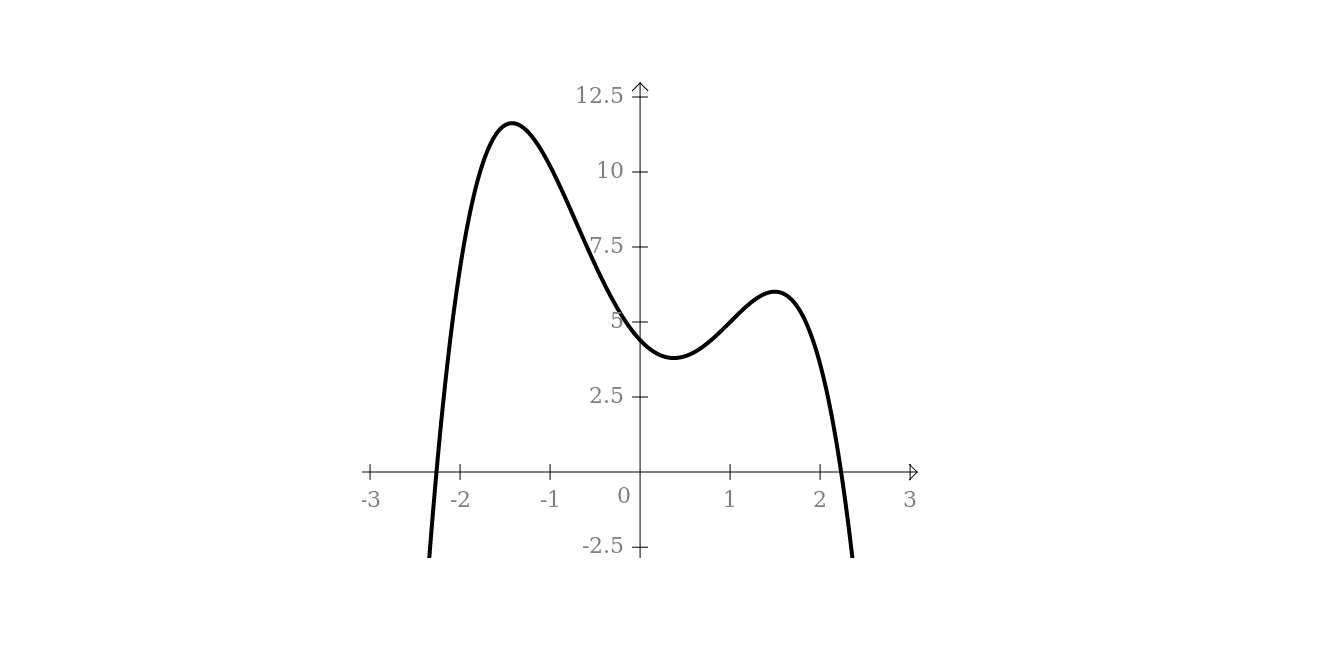
\includegraphics[scale=0.30]{\imgdirfromsection/polinomio-quarto-grau.png}
  \caption{Gráfico da função $p_4$.}
  \label{fig:polinomio-quartico}
\end{figure}

Para cada gráfico, identifique se o grau $n$ da função polinomial correspondente é par ou ímpar, e qual o sinal 
de $a_n$.
\end{example}

\begin{solution}
  Note que, nas funções dos gráficos nas Imagens \ref{fig:polinomio-quadratico} e \ref{fig:polinomio-quartico},
  tem-se que, para $\modu x$ suficientemente grande -- isso é, para os maiores valores de $x$ ---, 
  $p(x)$ é positivo. 
  Se $n$ fosse ímpar, então $p(x)$ seria positivo para os maiores valores de $x$ e negativo para os menores (maiores
  em módulo), ou vice-versa, mas, como vimos, isso não é verdade. 
  Logo, para essas funções, $n$ é par. 
  Ademais, como, na função da Imagem \ref{fig:polinomio-quadratico}, $p(x)$ é positivo nos maiores valores de $\modu x$, 
  tem-se que $a_n$ também o é. Na função da Imagem \ref{fig:polinomio-quartico}, $p(x)$ é negativo nos maiores
  valores de $\modu x$. Consequentemente, seu $a_n$ é negativo.

  Nas funções dos gráficos nas Imagens \ref{fig:polinomio-identidade} e \ref{fig:polinomio-cubico}, temos que o 
  sinal de $p(x)$ nos maiores valores de $x$ é diferente do sinal nos menores valores de $x$.
  Se $n$ fosse par, então o sinal de $p(x)$ teria que ser o mesmo; a saber, o sinal de $a_n$.
  Logo, o valor de $n$ de cada uma dessas funções é ímpar.  
  A função cujo gráfico é mostrado na Imagem~\ref{fig:polinomio-identidade} é positiva nos maiores valores de $x$,
  o que quer dizer que $a_n$ é positivo. 
  Já a função da Imagem~\ref{fig:polinomio-cubico}, por outro lado, é negativa nos maiores valores de $x$.
  Assim, $a_n$ é negativo.
\end{solution}


Outros fatos que nos ajudam a traçar gráficos de funções polinomiais são:
%
\begin{itemize}
\item Se o grau de $p$ é maior do que o grau de outra função polinomial $q$, 
então para todo $x$ com valor absoluto suficientemente grande, 
tem-se $\modu {p(x)} > \modu{q(x)}$;
\item Sejam $x_1, x_2 \in \R$. Se $p(x_1) < 0$ e $p(x_2)>0$,
então, $p$ deve possuir uma raiz entre $x_1$ e $x_2$.
\end{itemize}

\begin{example}
Considere os polinômios $p(x) = x^7 $ e $q(x)=x^3$. 
Quando $0< \modu x < 1$, temos que $\modu {p(x)} < \modu{q(x)}$. 
Porém, quando $ \modu x > 1$, temos que $\modu {p(x)} > \modu{q(x)}$. 
Além disso, em ambos os casos, $p(-1) = q(-1) = -1 <0$ e $p(1) = q(1) = 1 >0$.
Assim, os polinômios possuem, cada um, ao menos uma raiz no
intervalo $(-1, 1)$ -- a saber, $x=0$.
\end{example}

\begin{figure}[H]
  \centering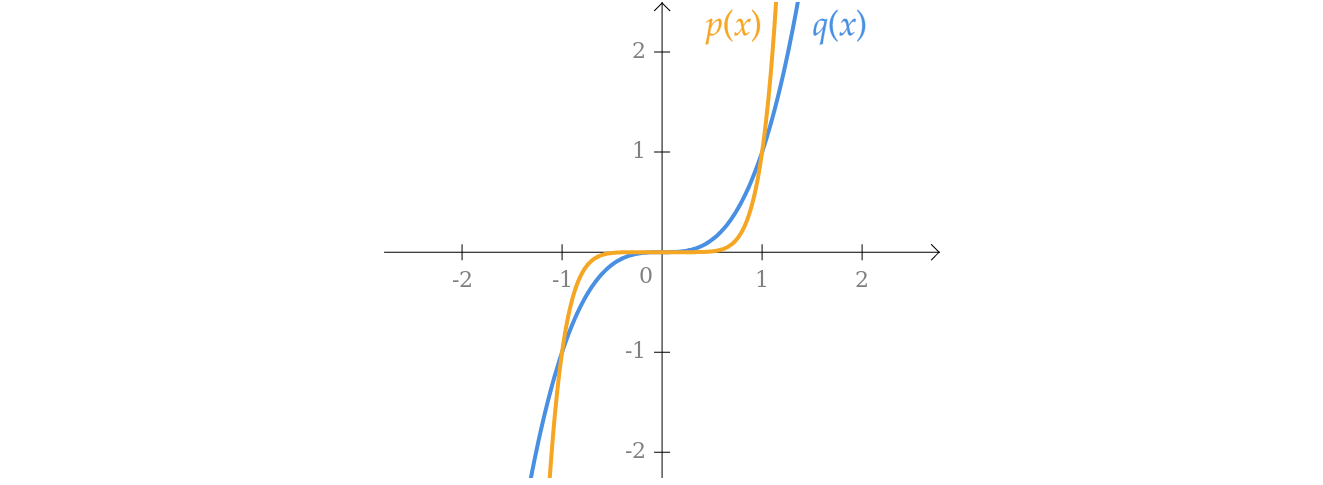
\includegraphics[scale=0.30]{\imgdirfromsection/raizes-em-um-intervalo.png}
  \caption{Gráfico das funções $p$ e $q$.}
  \label{fig:raizes-em-um-intervalo}
\end{figure}

\begin{onlineact}
    \khan{https://pt.khanacademy.org/math/algebra2/polynomial-functions/zeros-of-polynomials-and-their-graphs/e/using-zeros-to-graph-polynomials}
    {Zeros de Polinômios e seus Gráficos}.
\end{onlineact}